%TODO
% add figure references
% finish conclusion
% add diaphragm and bronchial tree closeups
% review reference ordering

\documentclass[letterpaper]{article}
\usepackage{ms1report}
\usepackage[pdftex]{graphicx}
\usepackage{times}
\usepackage{helvet}
\usepackage{courier}
\usepackage[numbers]{natbib}
\raggedbottom

\pdfinfo{/Title (The Nature of Breath) /Author (Lauria Clarke)}

\title{The Nature of Breath: A Biomimetic Kinetic Sculpture that Breathes}
\author{Lauria Clarke\\ Parsons School of Design, The New School\\ New York, USA\\ clarl404@newschool.edu\\}
\setcounter{secnumdepth}{0}

\begin{document} 
\maketitle

\begin{abstract}
The Nature of Breath is a kinetic sculpture exploring the sound and mechanics of human breath. By mimicking the mechanics of the human body this piece asks what it means for a machine to breath, drawing an uncertain line between what is considered natural and artificial and what is considered to be living or non-living. The Nature of Breath is also situated in response to the COVID-19 pandemic. In response to the virus' spread over the last two years, humans around the globe have become unusually attuned to the degrees of health or sickness that breath can indicate as well as the factors that may change one to the other. Through its contrast between the natural and artificial, this works intends to spur reflection on the pandemic as an indicator of humanity's relationship with the natural world. 
\end{abstract}

\keywords{Keywords}
kinetic sculpture, COVID-19, biomimicry, breath
%------------------------------
\section{Introduction}

% general introduction
% RANDOM NOTES AND OUTLINE
% Life is tghe avoidance of entropy - an indisputable natural law of the universe, therefor its opposite, life is as well (quote from zimmer).
%  -- is often tied up in kinetic sculpture. 
% layering the distinctions between what is natural and artificial and what is living and non-living.    
% 
% Movement is a natural indicator of life which situates kinetic sculpture as an ideal lens for invetsigating this blurred boundary between the natural and artificial.    
%   
% kinetic sculpture often blurs the line between what is natural and artificial using movement
% it's important that we think about this because the natural world is chnaging at an unprecidented rate
% there is something inherently natural about movement
% things thta move tend to be alive
% this is a basic distinction human beings have evolved to make - between living and nonliving
% through movement there is a deep relationship bewteen what is natural and what is or has been alive
% this work uses the movement of breath to explore this relationship
% CONCLUSION:
% Using the human act of breathing as a lens, this work attempts to lay a foundation for inquiry into the relationship between what is considered to be natural and what is or has been alive. While the focus of this work is on a specifically human form of breath, respiration in broader context is omnipresent in living organisms and is therefore an apt biological process with which to address this question. This machine may breath in a natural way, but its appearance clearly identifies it as something which is purely artificial.
% With each human breath on this planet we move deeper into the anthropocene.
% Respiration in breathing organisms is a visibly mechanical process. 
% Humans have created many mechanisms to mimic various aspects of the respiratory system for purposes ranging from medical devices, underwater exploration, to speech synthesis and more. Most of these devices are highly specialized and seek to mimic particular aspects of respiration such as oxygen delivery, or vocal modulation. These works rarely mimic the actual mechanics of the components of the human body responsible for respiration favoring more abstracted and efficient mechanical systems to achieve their goal. Using the freedom afforded by kinetic sculpture, this work attempts to blend a human-biomimetic approach -- highlighting the mechanical simplicity of the human body -- with a highly technical approach which allows for precise and complex control over the resulting breath. 

% art history reference https://thekeep.eiu.edu/cgi/viewcontent.cgi?article=4843&context=theses

% Art has been used as a medium to reflect and celebrate the beauty of the natural world for a long time. [need sentence here tying to the next paragraph]
%As the machine age took hold of the public's imagination and facility with mechanical devices became wide-spread, artist began to turn to medium of movement to reflect the natural world CITE. The birth of modern computing has made small, easy to use, and low voltage electronics increasingly accessible, allowing a new crop of artists to create even wider range of movement for mirrorig the complex beauty of movement in the natural world. 

Kinetic sculpture can be an incredibly powerful technique for re-contextualizing the beauty of movement often overlooked in everyday life. The process of recreating natural movement through mechanical, man-made means allows artists to highlight and isolate natural movement outside of its conventional context in nature. Mimicking the movement of a field of wheat in the wind, for example, draws our attention from the awe-inspiring scale of such a landscape to focus on the magical quality of movement produced by a single stalk operating within a group. While isolating such an innate quality of the natural world is itself magical, those looking a little closer cannot help but notice the stark contrast between such a natural movement and the artificial way in which it may be achieved. This blurred distinction between the natural and the artificial is a hallmark characteristic of biomimetic movement from kinetic sculpture to engineering and beyond. 

Our present understanding and knowledge of the natural world and it boundaries is changing at an unprecedented rate due to human caused environmental change. The question of what is natural and what has been altered, enhanced, or created by humankind -- the artificial -- is therefore increasingly urgent and difficult to answer. Through the lens of this question it becomes clear that creating a solid boundary between humankind and the rest of the natural world is a mindset which cannot be sustained indefinitely.\cite{smith} As Jedediah Purdy notes, ``the natural and the artificial have merged at every scale...If Nature were a place, we could not find it. If Nature were a state of mind, we could not attain it. We are something else, and so is the world.''\cite{purdy}

The question of what it means to be alive is unavoidable when considering the relationship between movement and what is natural. Movement is a key indicator of life and the ability to distinguish between the living and non-living is a deeply rooted capacity of the human brain. Psychologists and Neurologists have long been aware that ``the distinction between living and non-living things forms a natural place,'' to divide the functionalities and capacities of the mind.\cite{narine} Kinetic sculpture layers these two distinctions -- between the natural and the artificial and the living and non-living -- in an open-ended way which scientific disciplines are rarely allowed.   

Perhaps the most natural indicator of life is the movement of breathing. Respiration is an indicator of life at all scales - from single celled organisms to human beings. Whether involving oxygen in the conventional sense of breath, or operating at the cellular level, the process of energy production -- often for the purpose of movement -- is essential to life as we know it.\cite{zimmer} Taking breath, the most natural of human movements, into close consideration, this work examines the relationship between what is natural and what is, or has been, alive. This mechanism may breathe in a natural way, but its appearance clearly identifies it as something which is purely artificial. There is no question that this breathing work does not actually posses life.   

This work also asks us to consider the fragility of human breath in light of the COVID-19 pandemic. Seemingly overnight, much of the world became obsessed with breath as the toll of the virus spread. In the two years since, we have become incredibly attuned to the quality and sound of our own breath and what it may say about our mortality. This work seeks to probe these newfound sensitivities, forcing us to question which actions may lead the act of breathing to be easy or sharply painful. 
% Something about being alive. \cite{zimmer}

\subsection{Prior Work}
% talk about the history of breathing apparatus and note that none mimic the human body
Two notable works in the field of kinetic sculpture provide some reference and context for this work, Maywa Denki's WAHHA GO GO and Rafael Lozano-Hemmer's Vicious Circular Breathing.\cite{denki}\cite{lozanohemmer} 

Denki's work is arguably the more mechanically sophisticated of the two and most relevant in the discussion of breathing noises. WAHHA GO GO uses a bellows to force air through a larynx like opening which expands and contracts producing a laughing noise. The translation of motion through this piece is done using extremely precise and well made metal parts. This means that little noise -- aside from a pleasant whirring sound -- is generated by the mechanism itself focusing all of the viewers' attention on the eerie laughter it produces.

\begin{figure}[h]
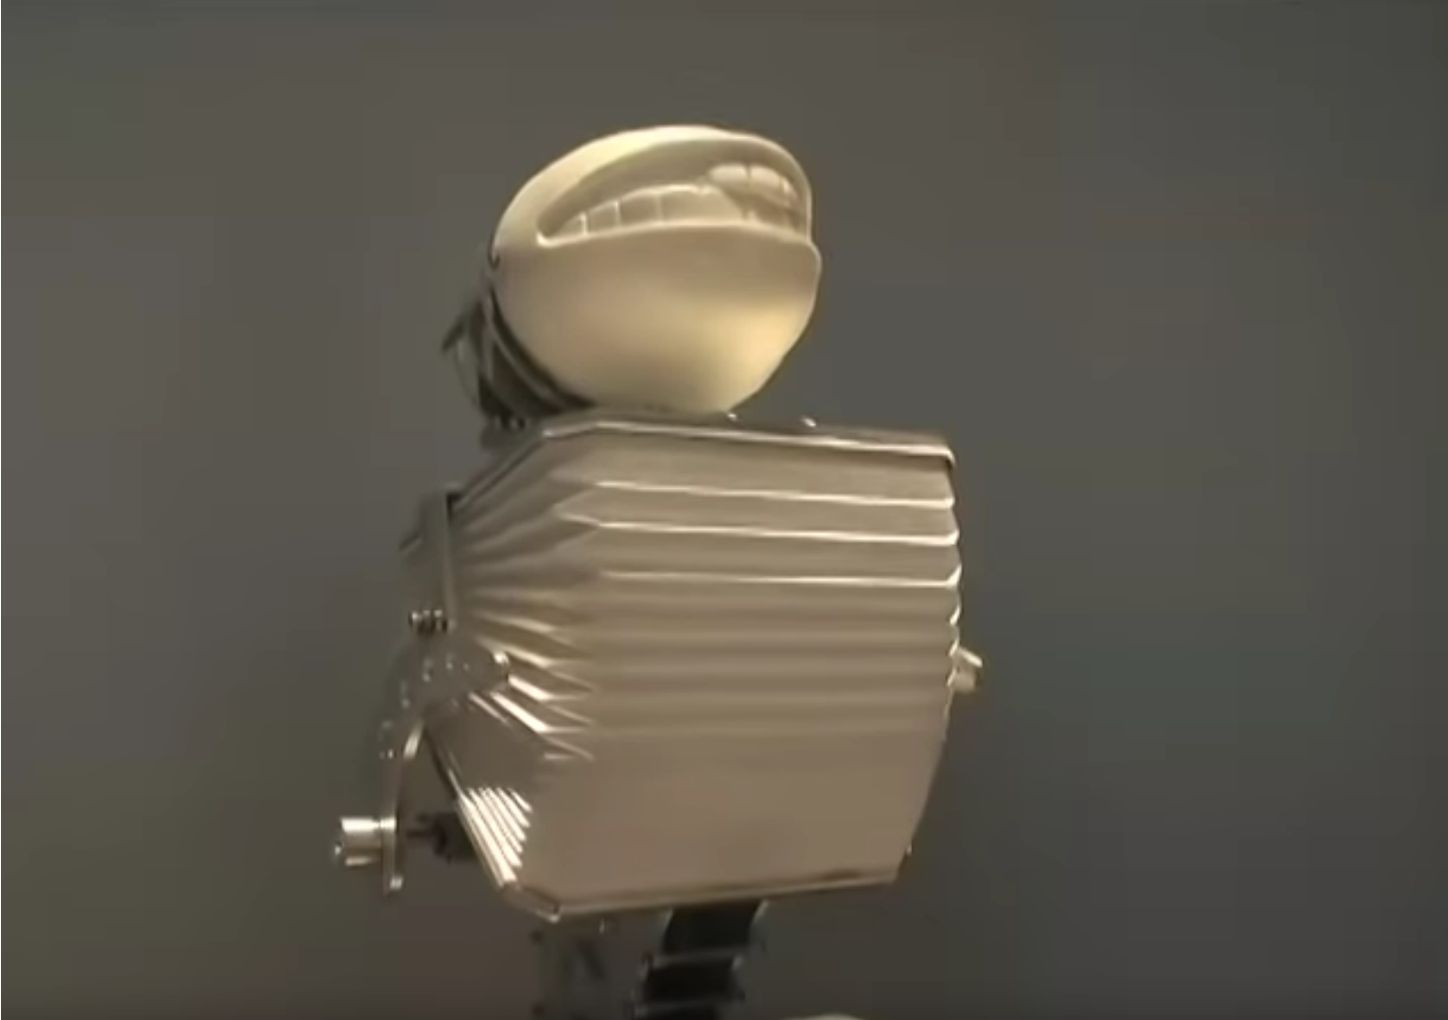
\includegraphics[width=0.5\textwidth]{images/whagogo.png}
\caption{WAHA GO GO by Maywa Denki}
\label{fig:denki}
\end{figure}

\begin{figure}[h]
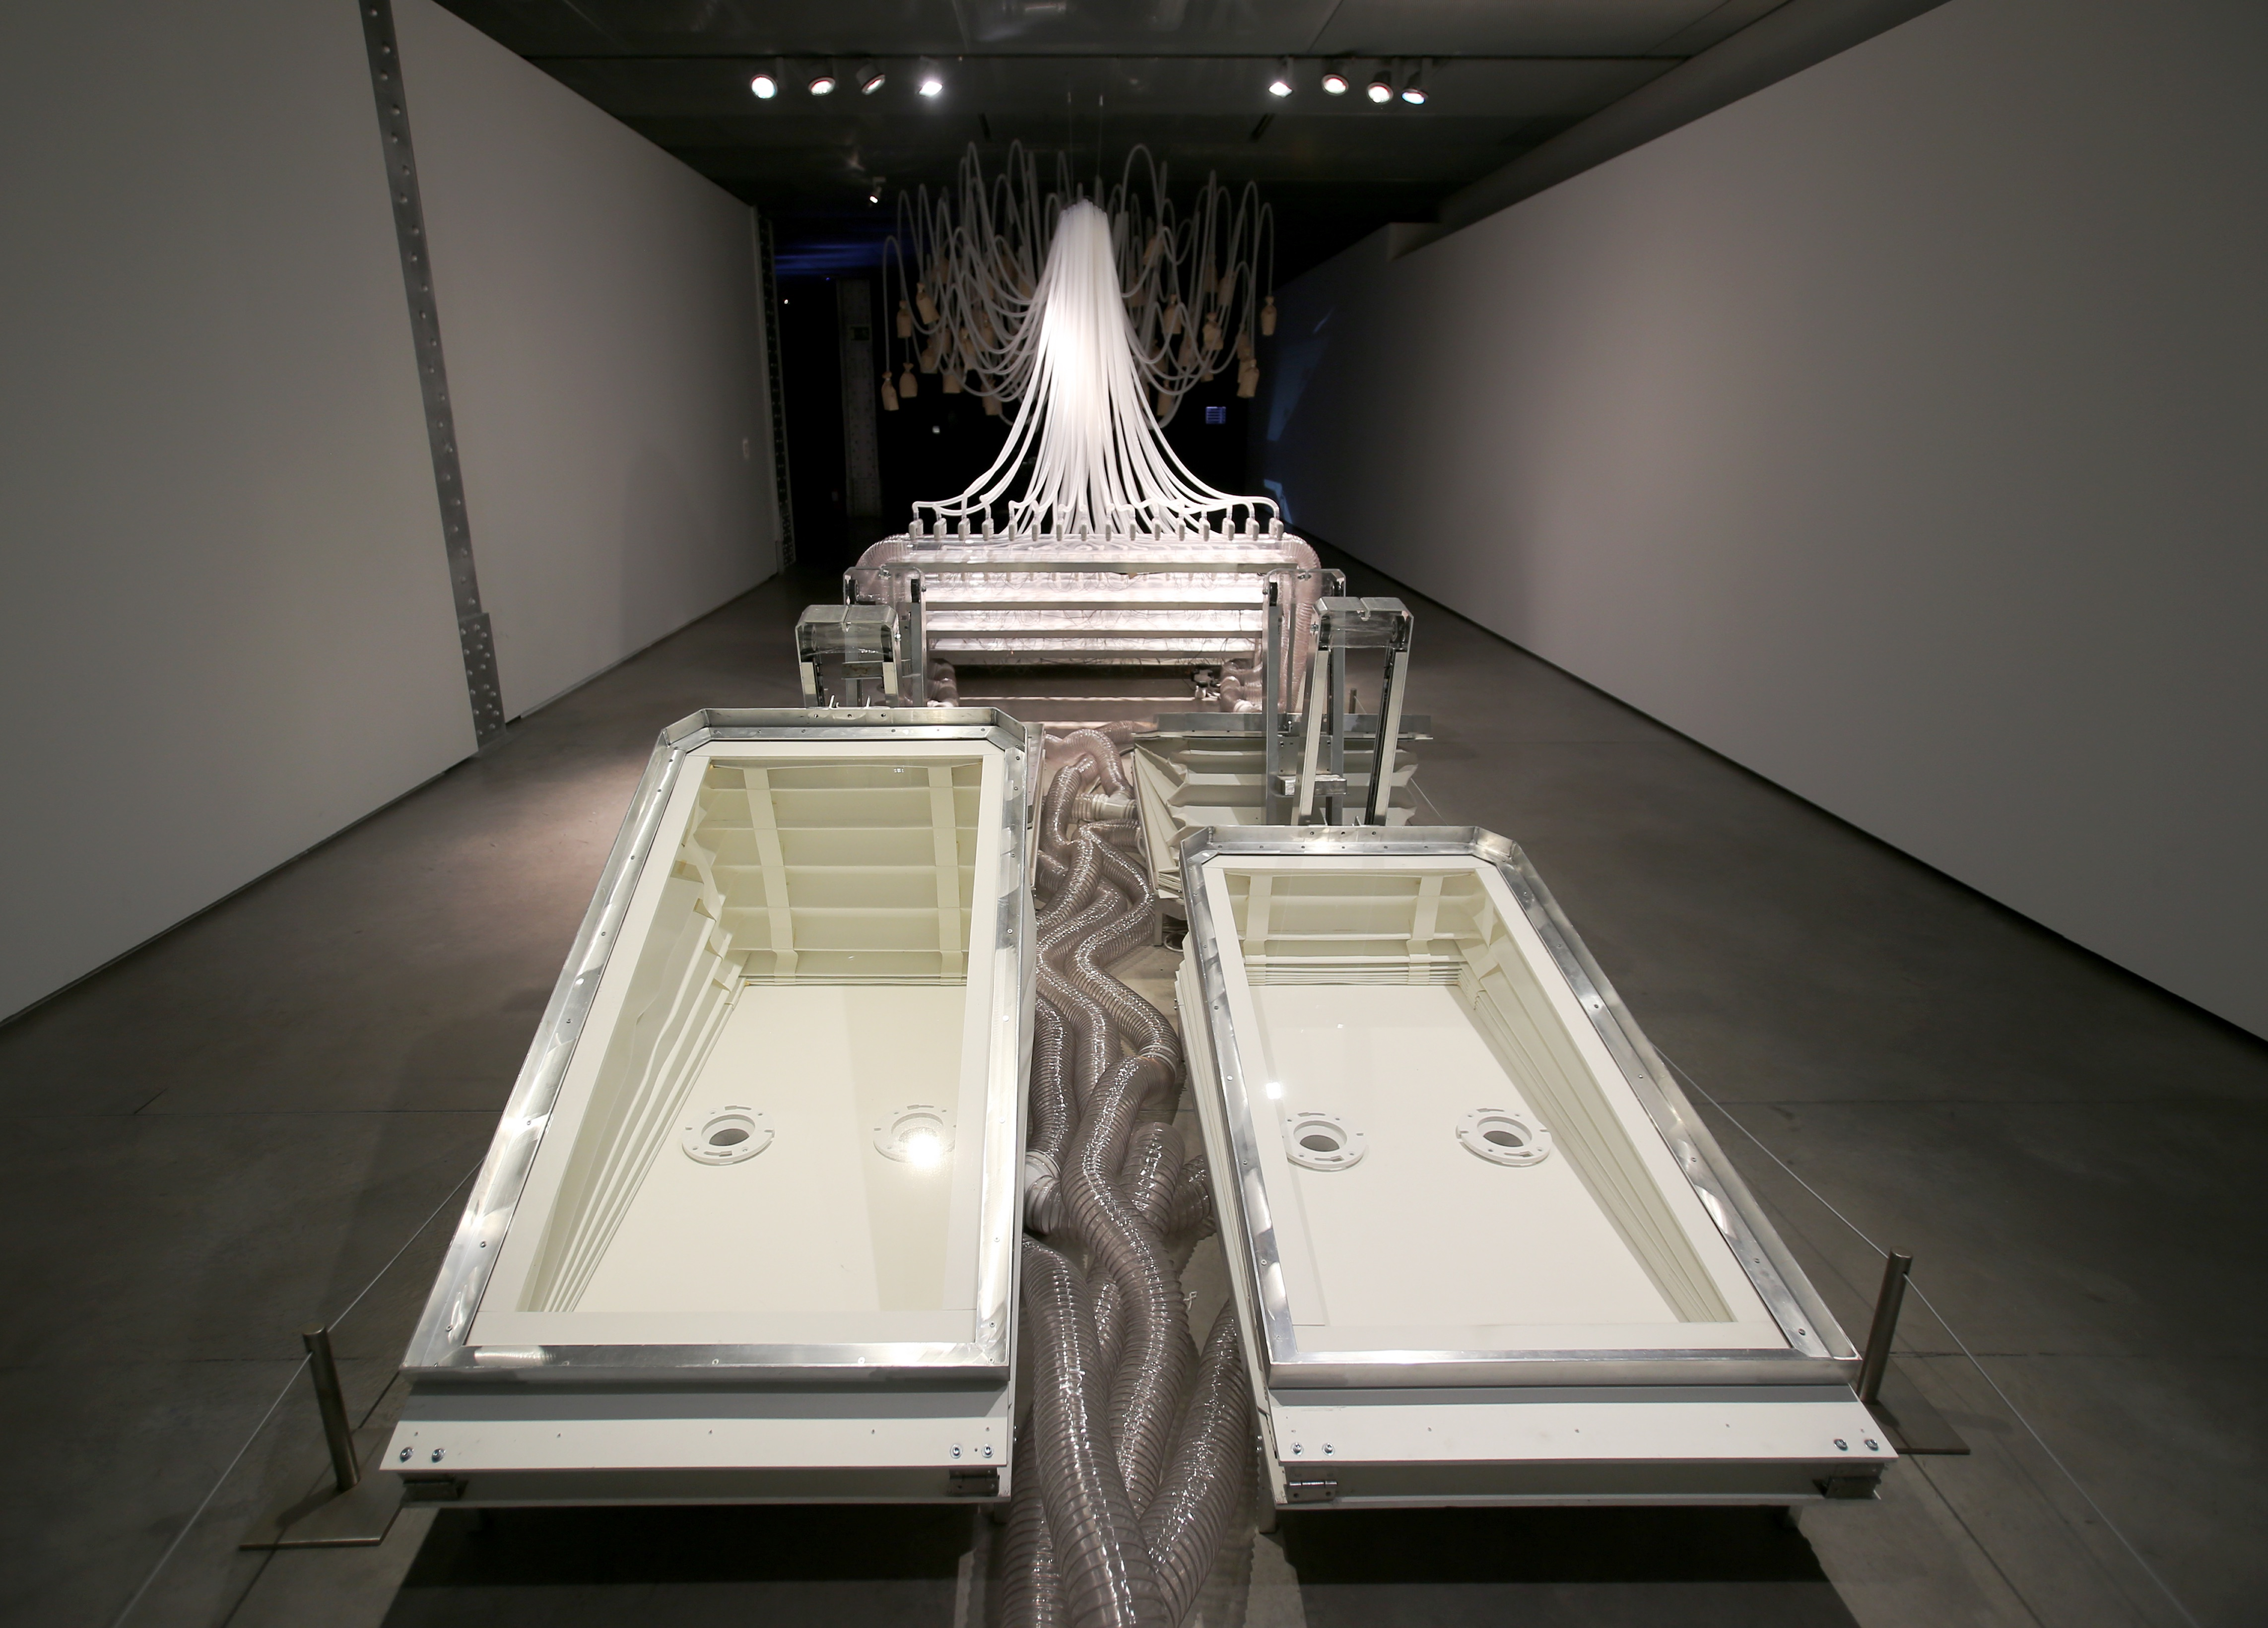
\includegraphics[width=0.5\textwidth]{images/vcb_madrid_2014.jpg}
\caption{Vicious Circular Breathing by Rafael Lozano-Hemmer}
\label{fig:hemmer}
\end{figure}


In contrast, Vicious Circular Breathing relies on the sharp sound of crinkling paper bags to indicate the movement of breath. This behemoth machine composed of gigantic bellows, yards of tubing, and a huge array of relays makes a lot of noise. Lozano-Hemmer's interest in breath is less about its bodily mechanics and more about the impacts and (un)sustainability of human breathing. Users are invited to add their breath to the closed loop system which eventually approaches a level of CO$_2$ saturation, rendering the piece unusable. Ultimately this sends a darker message about human breath.

These two pieces provoke thought about breath, but still use simple bellow based mechanisms to produce airflow. Bellows have been used for a long time in mechanical ventilation. Mechanical ventilation, as used in medicine since the early 1900s, seeks to provide ``replacement of the respiratory muscles.''\cite{ventilatorhistory} This results in apparatuses that resemble the respiratory system only in the sense that they cause a regulated change in pressure which allows for oxygenation of the blood. These devices have no need for recreating the process by which breath sounds are actually produced. The field of biomimetic robotics has little use for such inquiry either -- respiration is not necessary for an electronic being and it is much easier to produce vocal noises digitally than mechanically. 

Finally, it would be an oversight not to mention the hundreds of engineers and makers who devoted much time and though to the development of OpenSource emergency ventilators during the beginning and worst months of the pandemic.\cite{read} Very few of these devices were ever used on patients, but the collective thought and conversation surrounding the mechanics of breath cannot be discounted as useless, if only as a poignant reminder of the body's mystery and vulnerability. 

\section{Implementation}

Before beginning construction of the breathing machine I made a cursory, but interesting investigation into some of the techniques used for creating pressure differentials of air in industrial processes. These were expensive, noisy, and ultimately lay outside the scope of this discussion. The intent of this work was to draw mechanical inspiration from the human body, so I began my inquiry there. 

\subsection{System Breakdown}

The complexity of the human respiratory system lies not in its gross mechanics, but in the biological materials and molecular mechanics that allow for the transfer of oxygen to the blood.\cite{gasexchangers} To simplify this system for translation to a constructable mechanical structure, I broke it down into three main sub-systems. Each sub-system exists solely for the purpose of generating breath noises and not for the actual exchange of oxygen as would normally occur during respiration.

\begin{figure}[h]
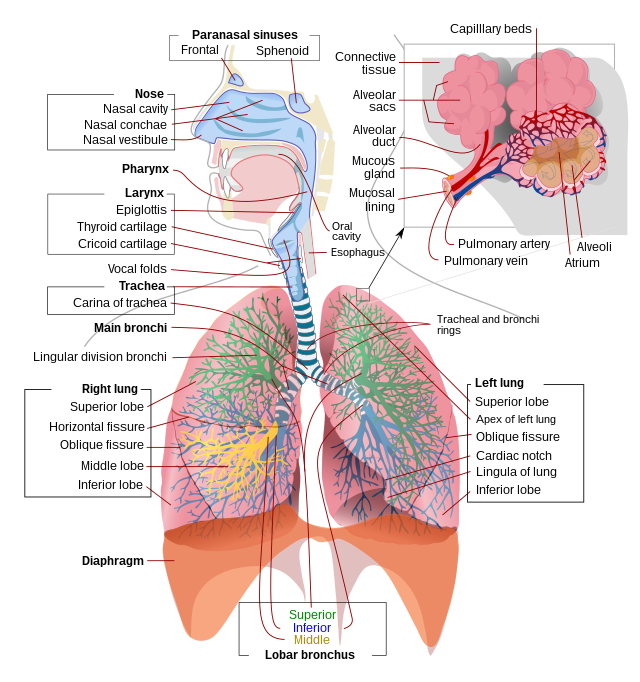
\includegraphics[width=0.5\textwidth]{images/respiratorysystem.png}
\caption{Diagram of the human respiratory system.}
\end{figure}

\subsubsection{Actuation}

Actuation is the process which causes air to move through the respiratory system. In our own bodies this is achieved by the movement of the diaphragm. In ventilators this is often achieved by a pump or bellows.

\subsubsection{Storage}

Storage describes the way air is stored and contained during the act of breath. This is done by the lungs and is only necessary for the transfer of oxygen to the blood. While the lungs are arguably the most critical part of the respiratory system, they are the most difficult to simulate with accuracy and have relatively little bearing on the sound of breath in this context.

\subsubsection{Modulation}

Modulation is the way the sound of breath is shaped as it leaves the body. This is achieved by the bronchial tree, trachea, larynx, pharynx, and mouth.\cite{sarkar} After actuation has been achieved, simulation of this system is the most relevant and interesting part of this project.   

\subsection{Making and Testing}

Focusing on the two main areas of inquiry, the making and testing has been divided into been auditory prototypes -- exploring the effect of disembodied breath noises -- as well as mechanical prototypes -- exploring ways to achieve a physiologically accurate breathing mechanism. In addition to creating a visual tie between the biological nature of the respiratory system, I chose to closely mimic the diaphragm and trachea to prevent the noise of the mechanical components from overwhelming the noise of the breath produced. This approach relies on the material properties of latex and vinyl -- elasticity and rigidity -- to be functional.

\subsubsection{Auditory Trials}

The objective of these prototypes was to understand the reaction observers have to disembodied breath noises. Disembodied in this case means that the noise is not coming from a source which appears to be alive. Some of this testing was done in a classroom with an audience who knew what was happening, and some was done on the streets of New York City with passersby. Both achieved surprisingly similar results. 

To test the effect of disembodied breath on strangers, a small speaker was placed inside of two five gallon plastic buckets. An old cellphone was pre-loaded with a three minute sound effect track of different types of breathing noises. These cycled through breath which sounded like someone sleeping to someone wheezing from exertion. In one bucket, a hole was drilled and a large diameter latex tube was inserted. This provided a way to direct the sound emanating from the speaker and added obfuscated the function of the assembly. The assembly was then placed near a crosswalk with a high level of foot traffic around 8 PM ET on the day of Halloween. This location was chosen specifically because it was easy to observe discreetly and had a wide variety of pedestrians. 

\begin{figure}[h]
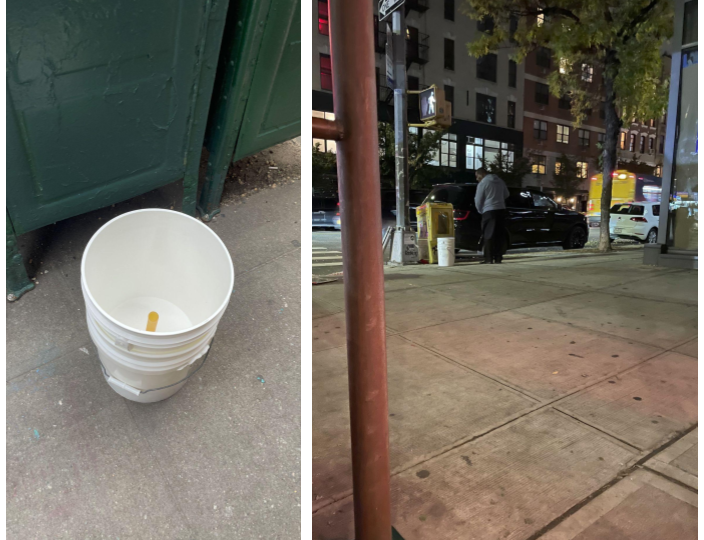
\includegraphics[width=0.5\textwidth]{images/buckettest.png}
\caption{Passerby observing a breathing bucket.}
\end{figure}

Due to the road noise of the location I only observed a handful of passersby alter their activity because of the bucket. It's possible many more heard the noise and simply ignored it. Those who did notice the noises were visibly confused or disconcerted and usually took a moment to look inside the bucket. It was clear based on this action that they were expecting something to be inside the bucket. The most interesting interaction happened while a young woman was waiting at the crosswalk with a group of friends. She happened to be near the edge of the group closest to the bucket and was clearly confused yet intrigued by the noise, as she kept looking furtively over her shoulder at the bucket. It was also clear that she felt some uncertainty or concern about the interaction because I observed that she didn’t immediately mention it to her companions.

The second investigation of disembodied breath happened in a classroom setting with a prepared audience. First, normal breath noises were played. Then, the noises of someone coughing and wheezing were overlaid at a much louder volume. Almost immediately, the audience was extremely uncomfortable with the ``sick'' noises. A few began to cover their ears. Due to the level of discomfort visible around the room I decided to end the experiment. A smaller version of this experiment was repeated at lower volume with an audience of only three people with similar results. There was immediate, visible concern among the audience when the ``sick'' breathing began to play.

\subsubsection{Physical Trials}

The objective of this second category of trials was to investigate ways of generating breathing noises mechanically. Using the systems breakdown discussed above, I attempted to create mechanisms for both modulation and actuation of breath. I first approached the diaphragm since actuation was a necessary step to fully explore modulation.

Using the five gallon buckets earlier, I cut out the center of the lid of one bucket and used it to secure a large piece of 25 mil natural latex over the opening. I then inserted the same large piece of latex tubing into a hole at the other end of the bucket. By depressing the latex air was forced out of the tube. Pinching the tube at different heights and changing the cadence of the diaphragm movement created a pretty wide range of breath-like noises. 

%\begin{figure}[h]
%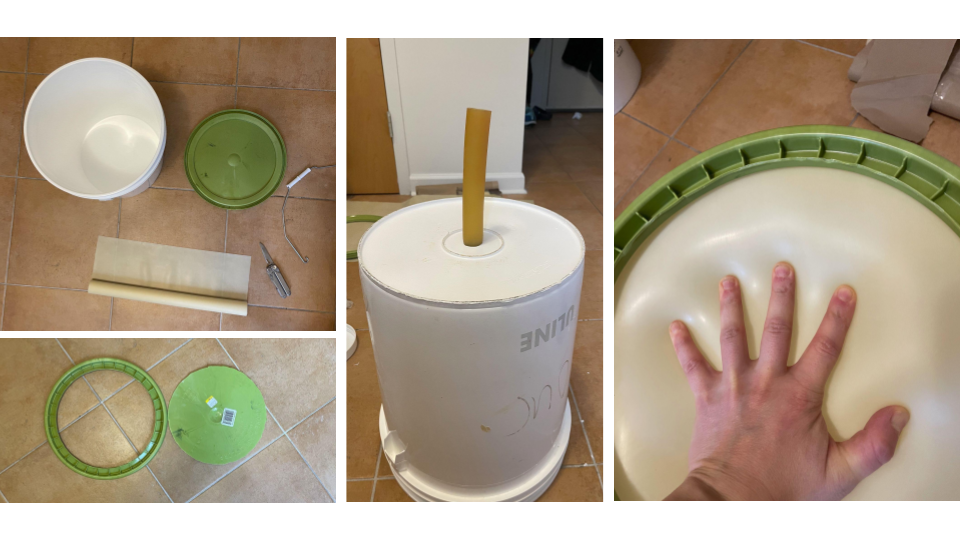
\includegraphics[width=0.5\textwidth]{images/diaphragm.png}
%\caption{Diaphragm and rudimentary trachea using five gallon bucket.}
%\end{figure}

This assembly was then mounted on a frame created using t-slotted aluminum. A lever was also installed under the diaphragm. The end of the lever had a long piece of metal wrapped in a soft rag which was roughly centered on the diaphragm. By depressing the lever with my foot the end of this lever extended into the diaphragm activating it while I used my hands to create variation in the noise of the airflow through the tube. This was sort of a ``playable'' breath maker. 

\begin{figure}[h]
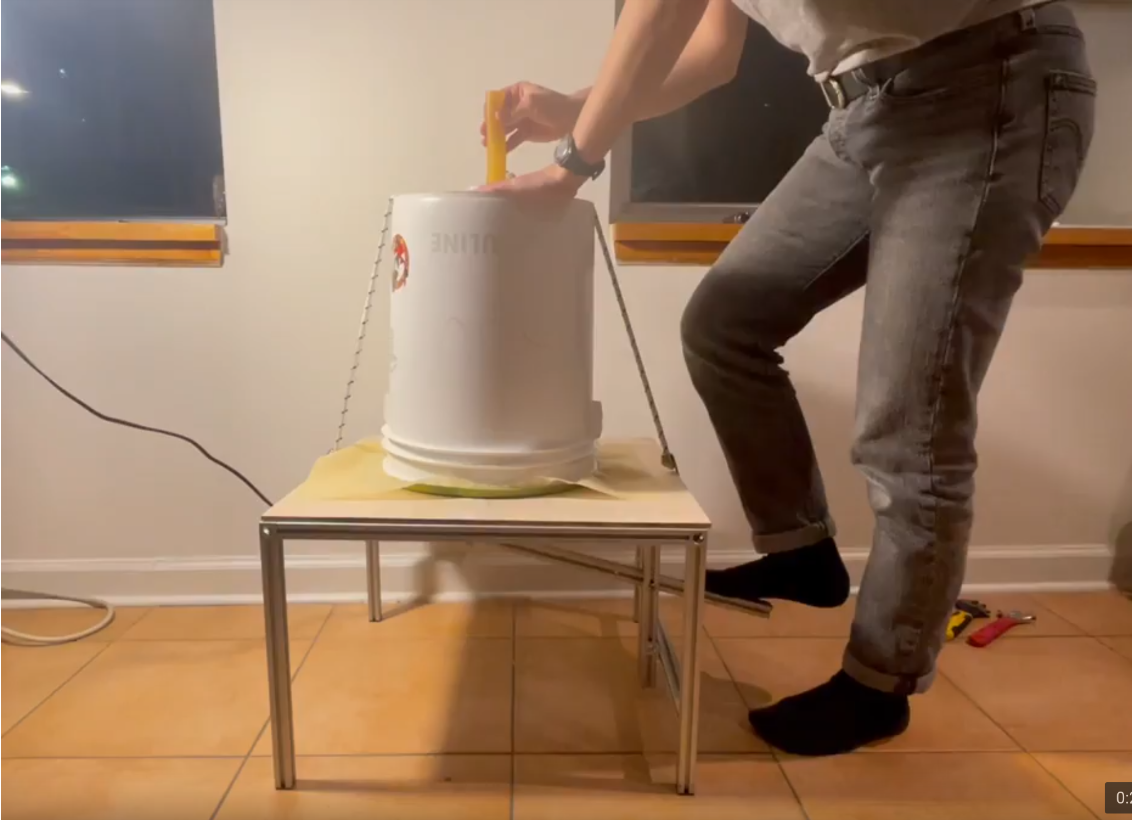
\includegraphics[width=0.5\textwidth]{images/playablebreath1.png}
\caption{Previous assembly installed with lever.}
\end{figure}

After measuring the force required to depress the lever fully -- 100 N -- I determined that creating an electronic system to activate the diaphragm would be costly and complicated given the scope of time. A few attempts at creating mechanical advantage for the lever were attempted, but none had successful results. It was very difficult to generate the required amount of force without putting a significant amount of weight on the lever itself. I ultimately decided that, due to the expense of high-powered and quiet motors, it made more sense to solve this problem after the core interaction of the piece had been refined. 

To approach modulation I decided to rely, again, on the mechanics of the human body. The trachea contains C shaped bands of cartridge with a section smooth muscle on the open side. When this muscle contracts the C shape is compressed changing how air flows through the trachea. The trachea is about one inch in diameter.\cite{furlow} I found that a two inch section of $1/8$ inch vinyl tubing had an internal radius of about one inch when bent in a C shape which reduced to less than a quarter of an inch when the two ends of the C were pulled together.  

\begin{figure}[h]
\centering
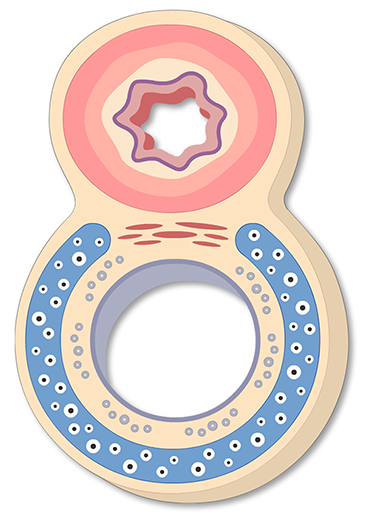
\includegraphics[scale=0.3]{images/trachea.png}
\caption{Cross section of the trachea and esophagus.}
\end{figure}

I embedded four sections of this tubing between two sheets of fourteen mil natural latex. I then bent this into a curved tube-like shape and enclosed the open end of the C FIG. Once this basic shape was complete I threaded each piece of tubing with monofilament and anchored the assembly between two dowels. By pulling on the monofilament is was possible to contract each ring within the tube individually. This result was highly successful and it was possible to contract the aperture to varying degrees.

\begin{figure}[h]
\centering
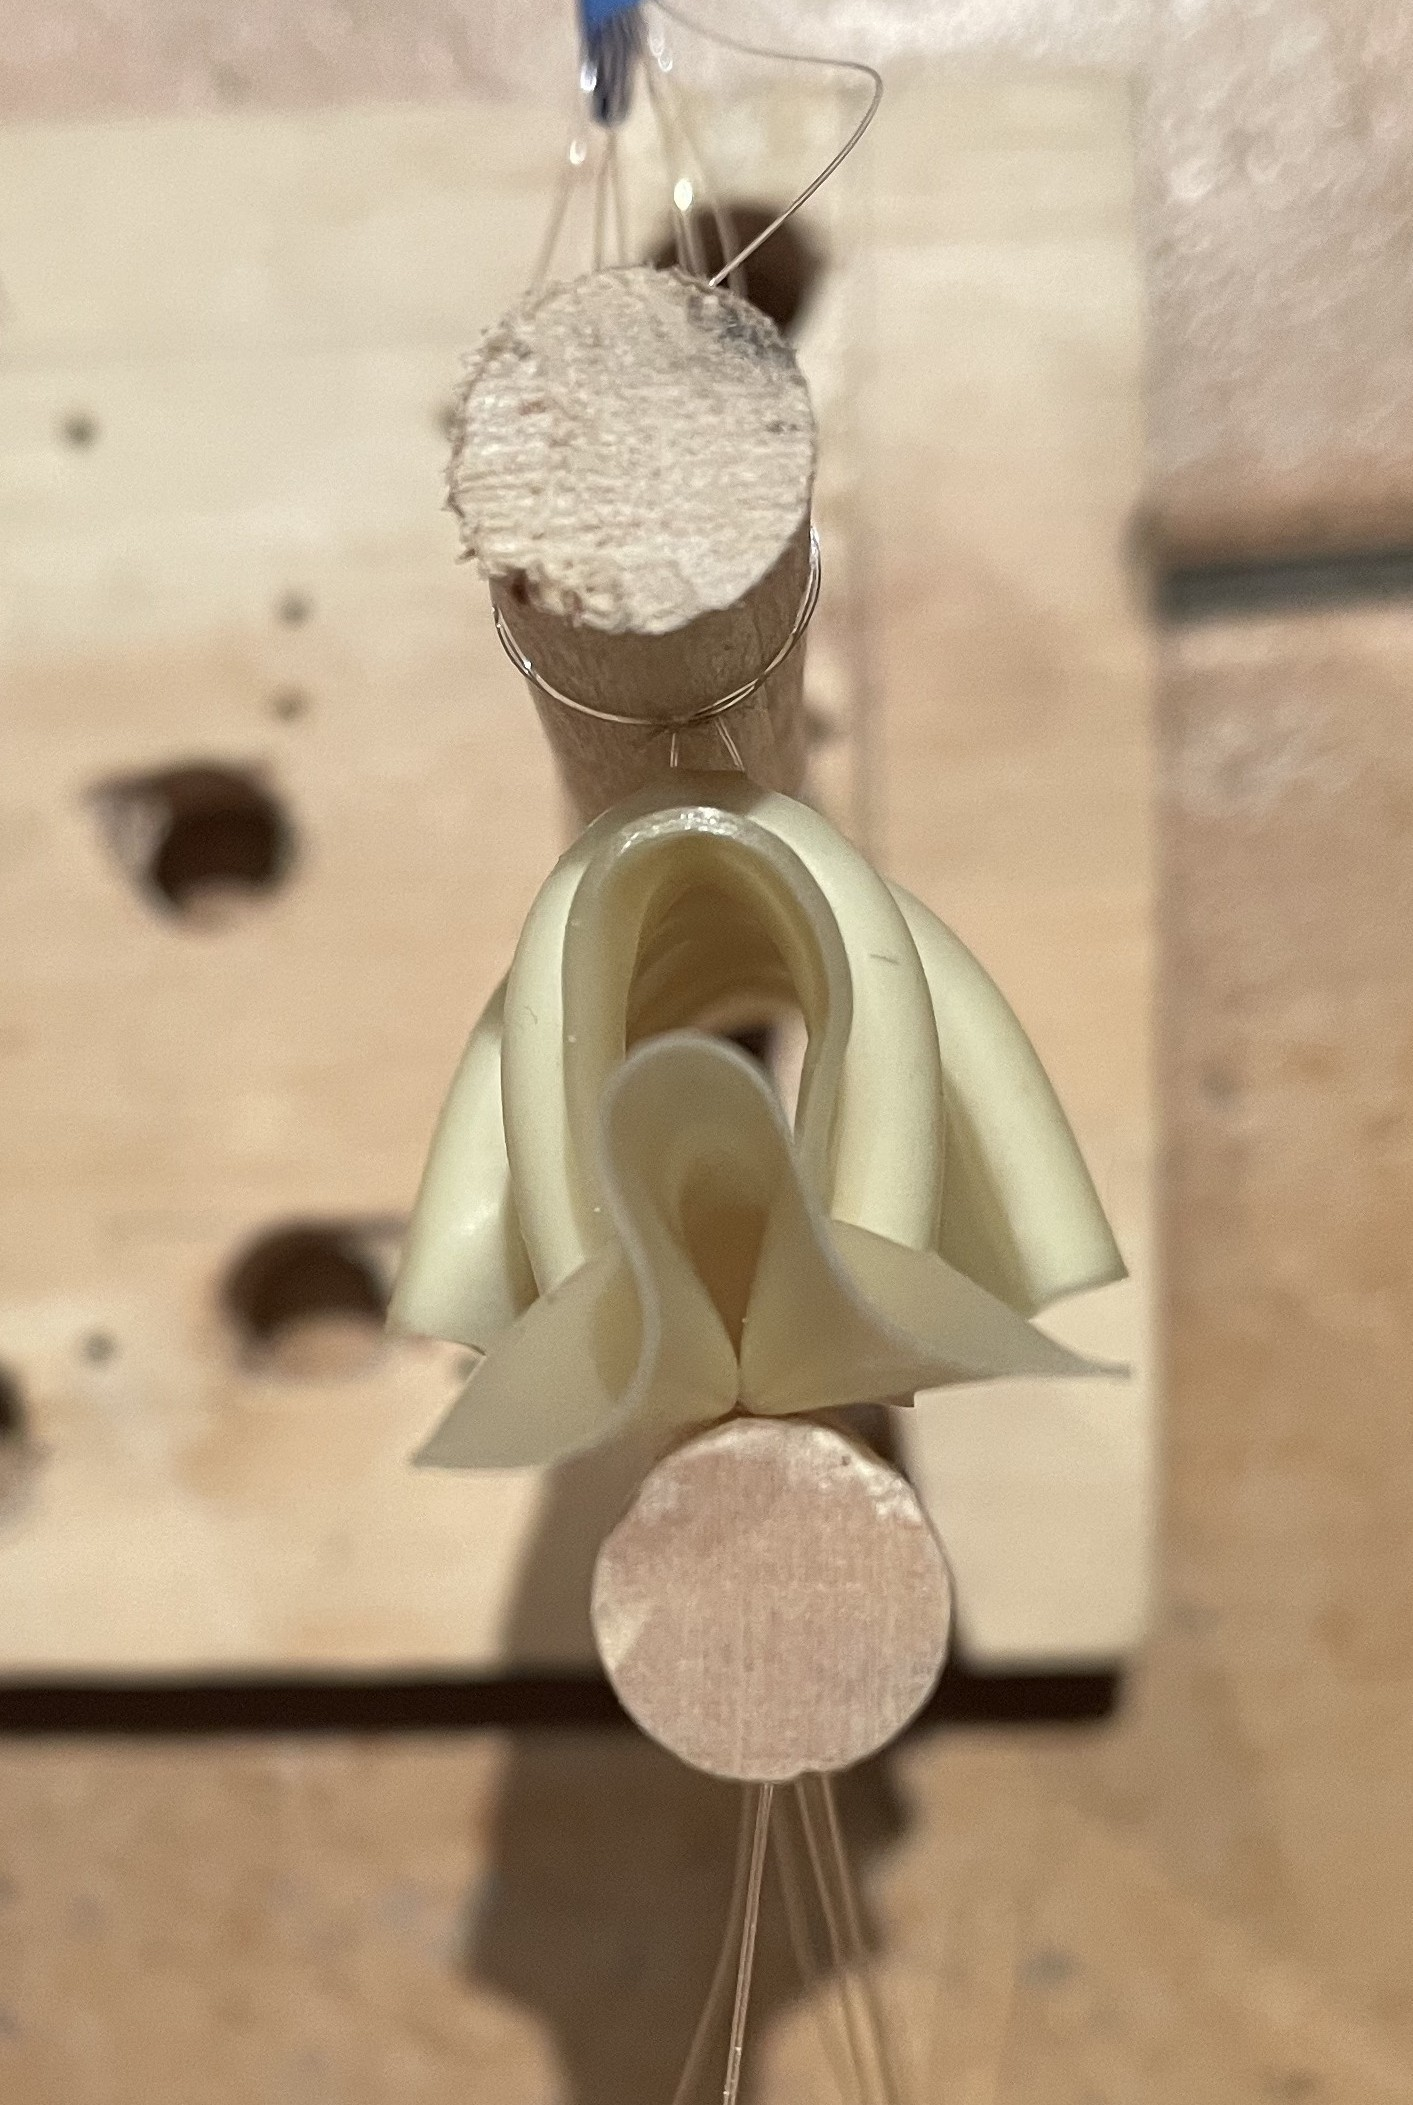
\includegraphics[width=0.22\textwidth]{images/46.JPG}
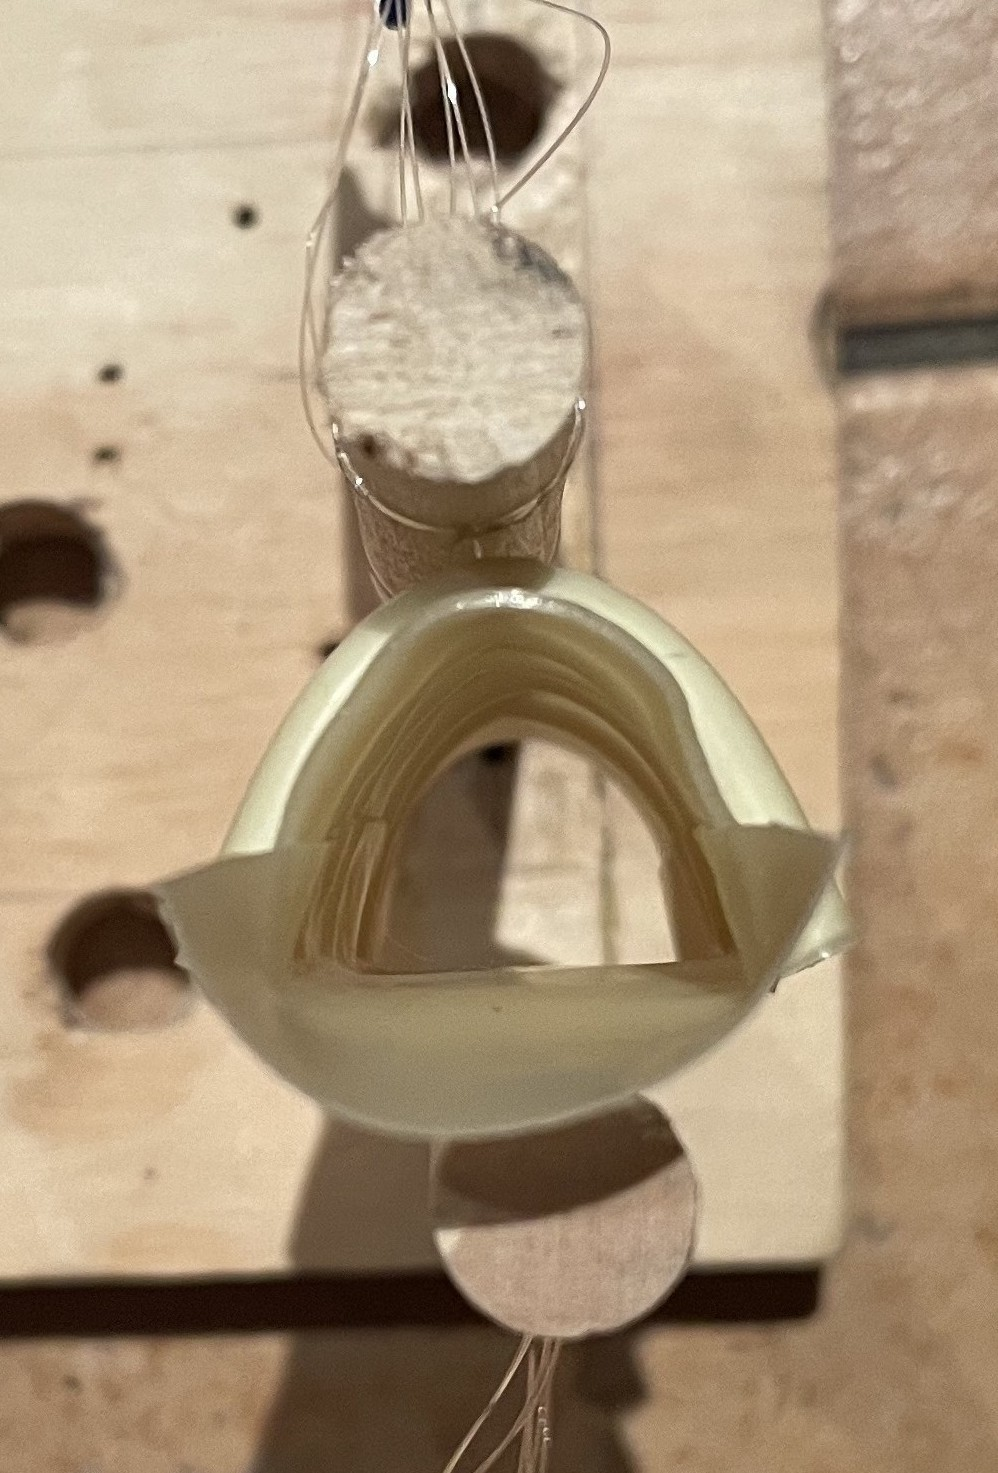
\includegraphics[width=0.22\textwidth]{images/52.JPG}
\caption{Contracted and relaxed trachea.}
\end{figure}

While this result was not integrated into the modulation prototype, it was by far the most naturalistic movement produced during the investigation. In comparison to the latex tubing used to mimic the trachea earlier, this mechanical latex assembly has much thinner walls. Overall, I believe this will produce more accurate breath noises when combined with the actuation mechanism

\subsubsection{Combined Trial}

Based on the results of the trials discussed above, I produced a final version combining the successful auditory and physical components.

I first created a digital breath generator in order to create a more nuanced interaction between the viewer and the breathing noises. This was done using P5.js and allowed me to change the cadence, pitch, and volume of the breathing noise. A simple infra-red distance sensor was then connected to the generator. As the distance between the viewer and the work decreased the breathing increased in intensity. The breath noise was amplified using a class D audio amplifier and played through speakers mounted on the front of the piece. 
 
%\begin{figure}[h]
%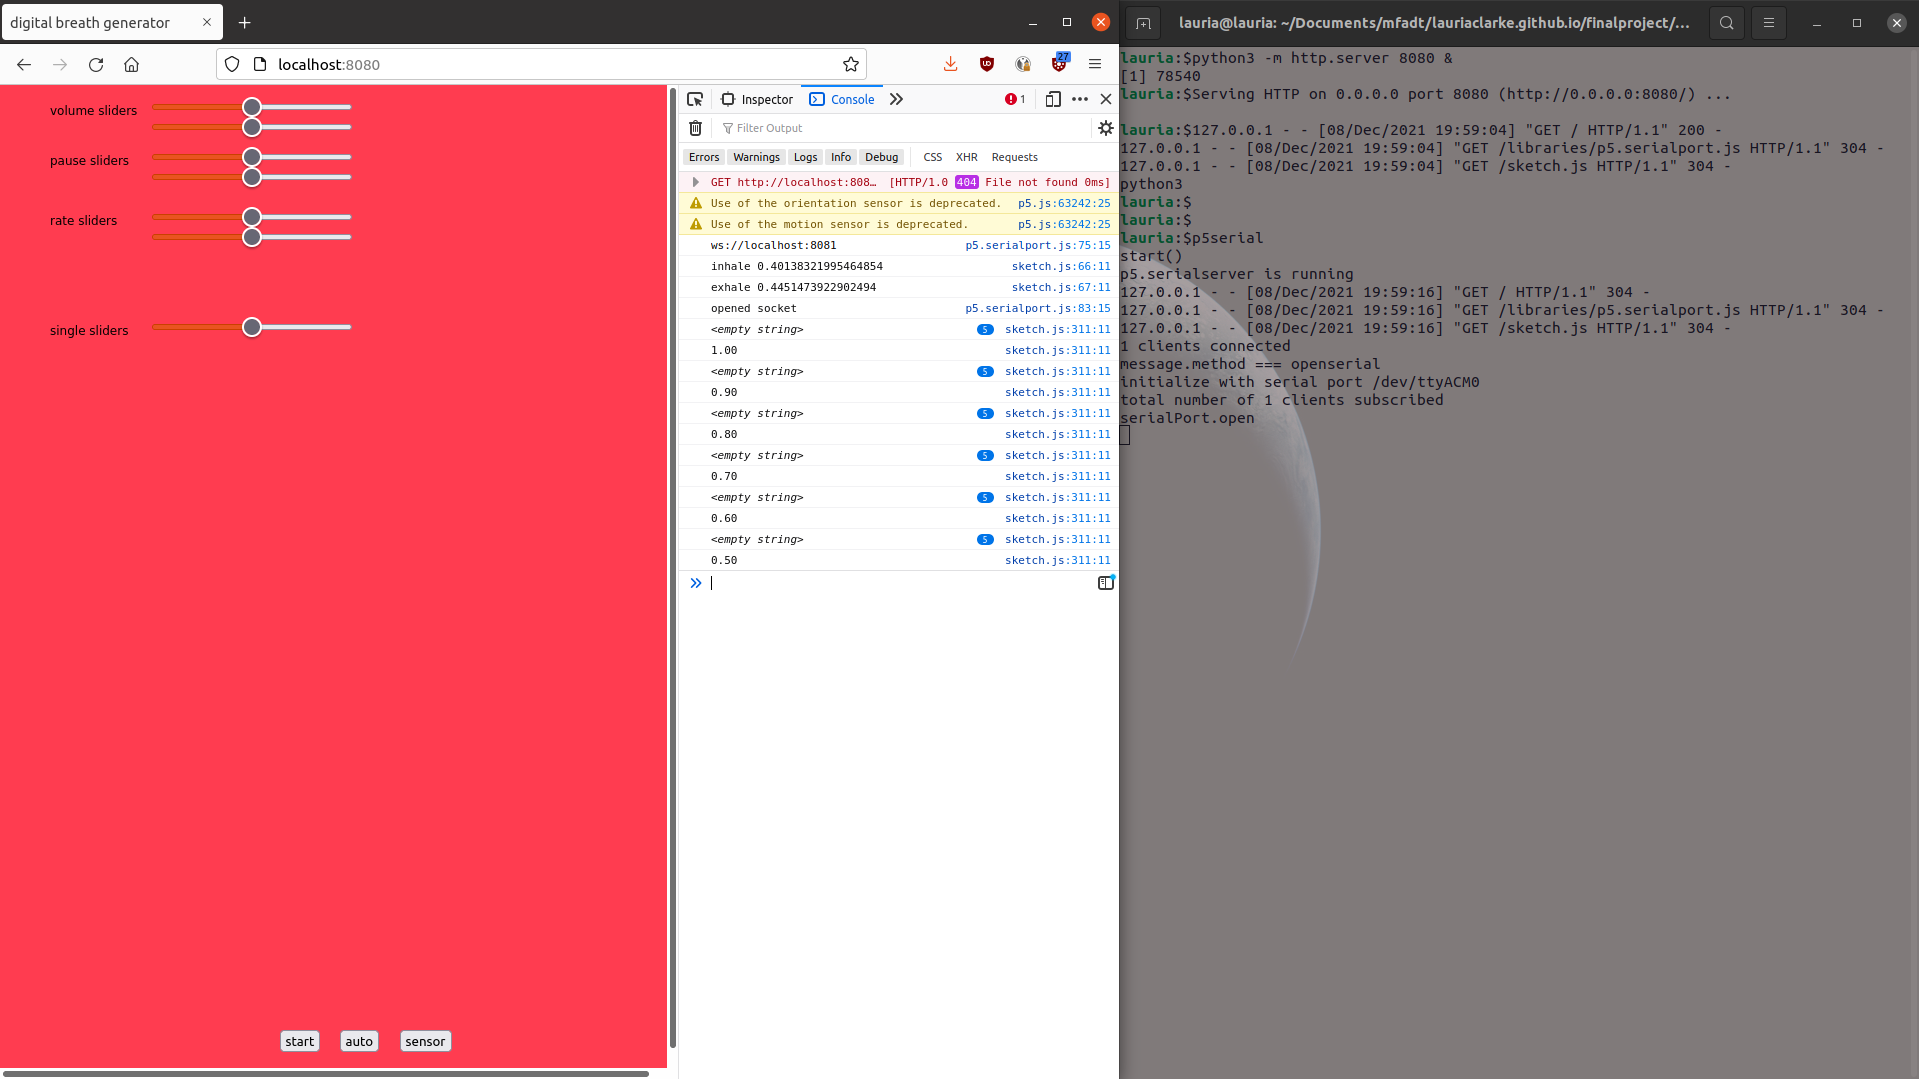
\includegraphics[width=0.5\textwidth]{images/digitalbreath.png}
%\caption{Digital breath generator.}
%\end{figure}

The mechanical form of the work stayed the same in this trial, however I removed the five gallon bucket in favor of a clear vessel which allowed the viewer to see the diaphragm moving. I also added an abstracted bronchial tree inside the vessel to suggest lungs. In combination with the added electronics this had a much more polished effect.

\begin{figure}[h]
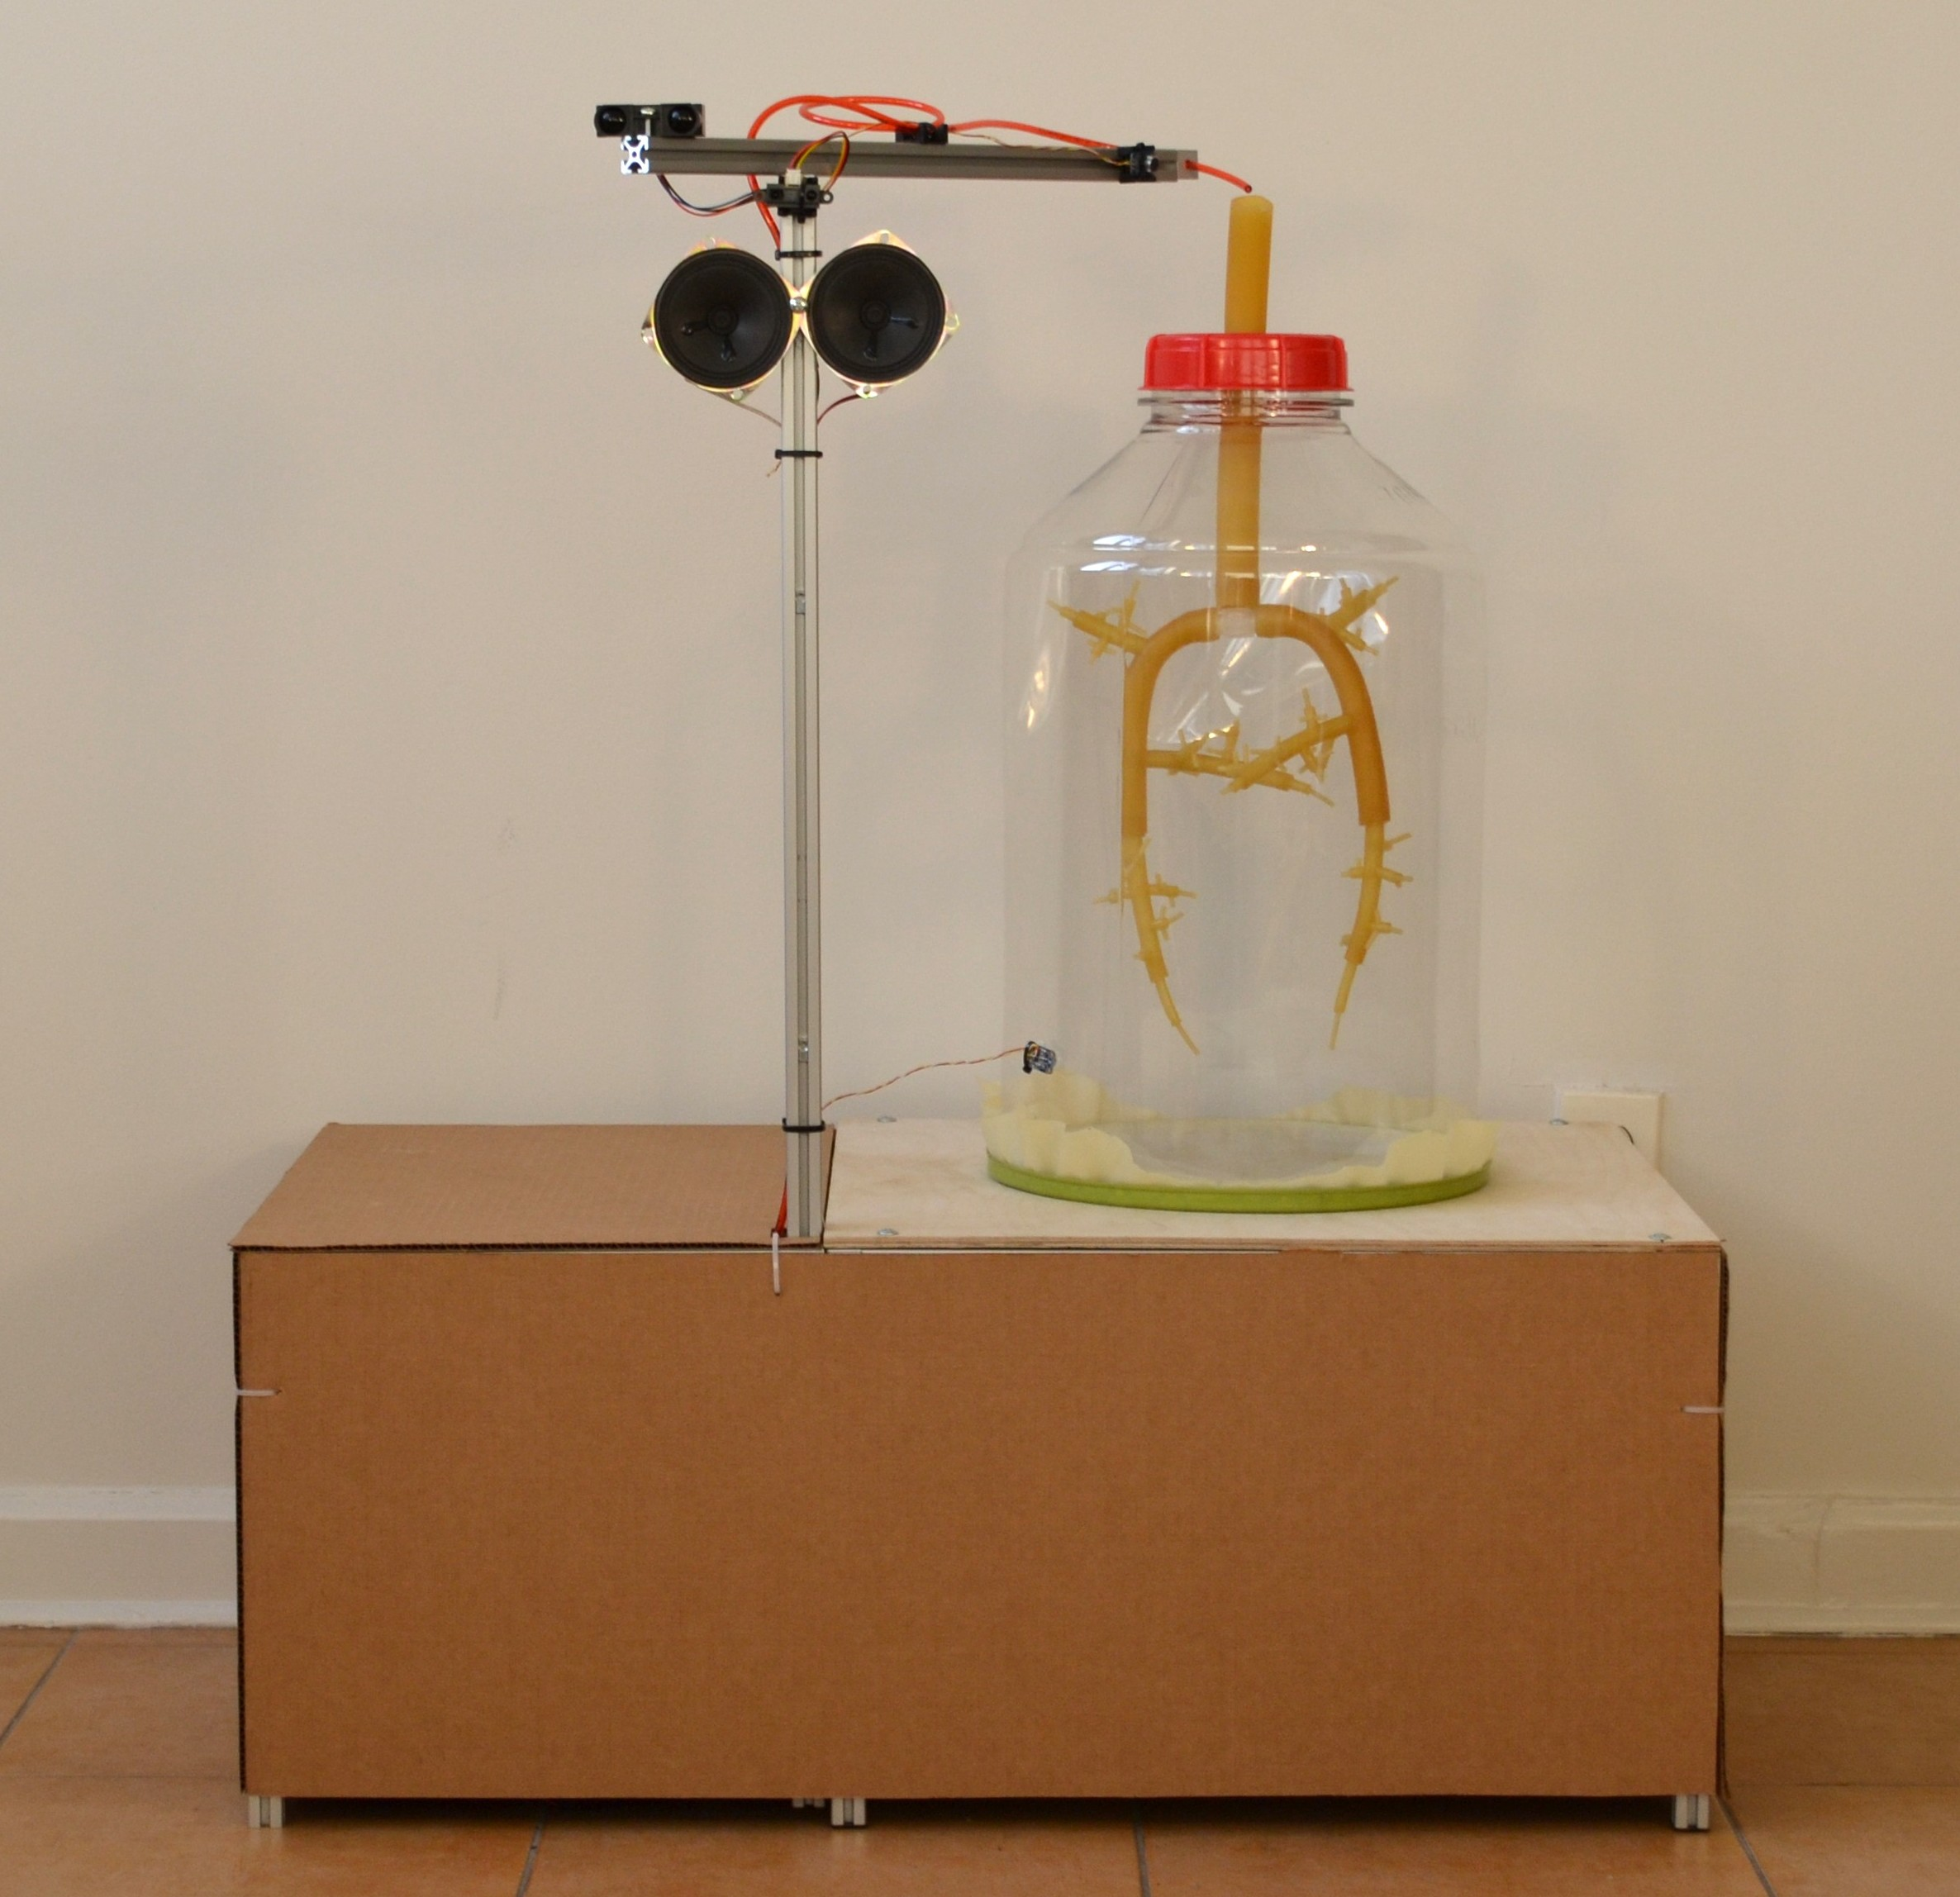
\includegraphics[width=0.5\textwidth]{images/finaltrial.JPG}
\caption{Final form with infra-red distance sensor and digital breath generator.}
\end{figure}


This trial was much more effective. The auditory component of the interaction was much more natural and made it easier to grab the viewer's attention. The visual appearance of the piece was also more interesting, making it easier to draw the connection between the object and the breathing noises produced. 

\begin{figure}[h]
\includegraphics[width=0.5\textwidth]{images/closeupdiaphragm.JPG}
\caption{Diaphragm being activated by lever.}
  \label{fig:denki}
\end{figure}

\begin{figure}[h]
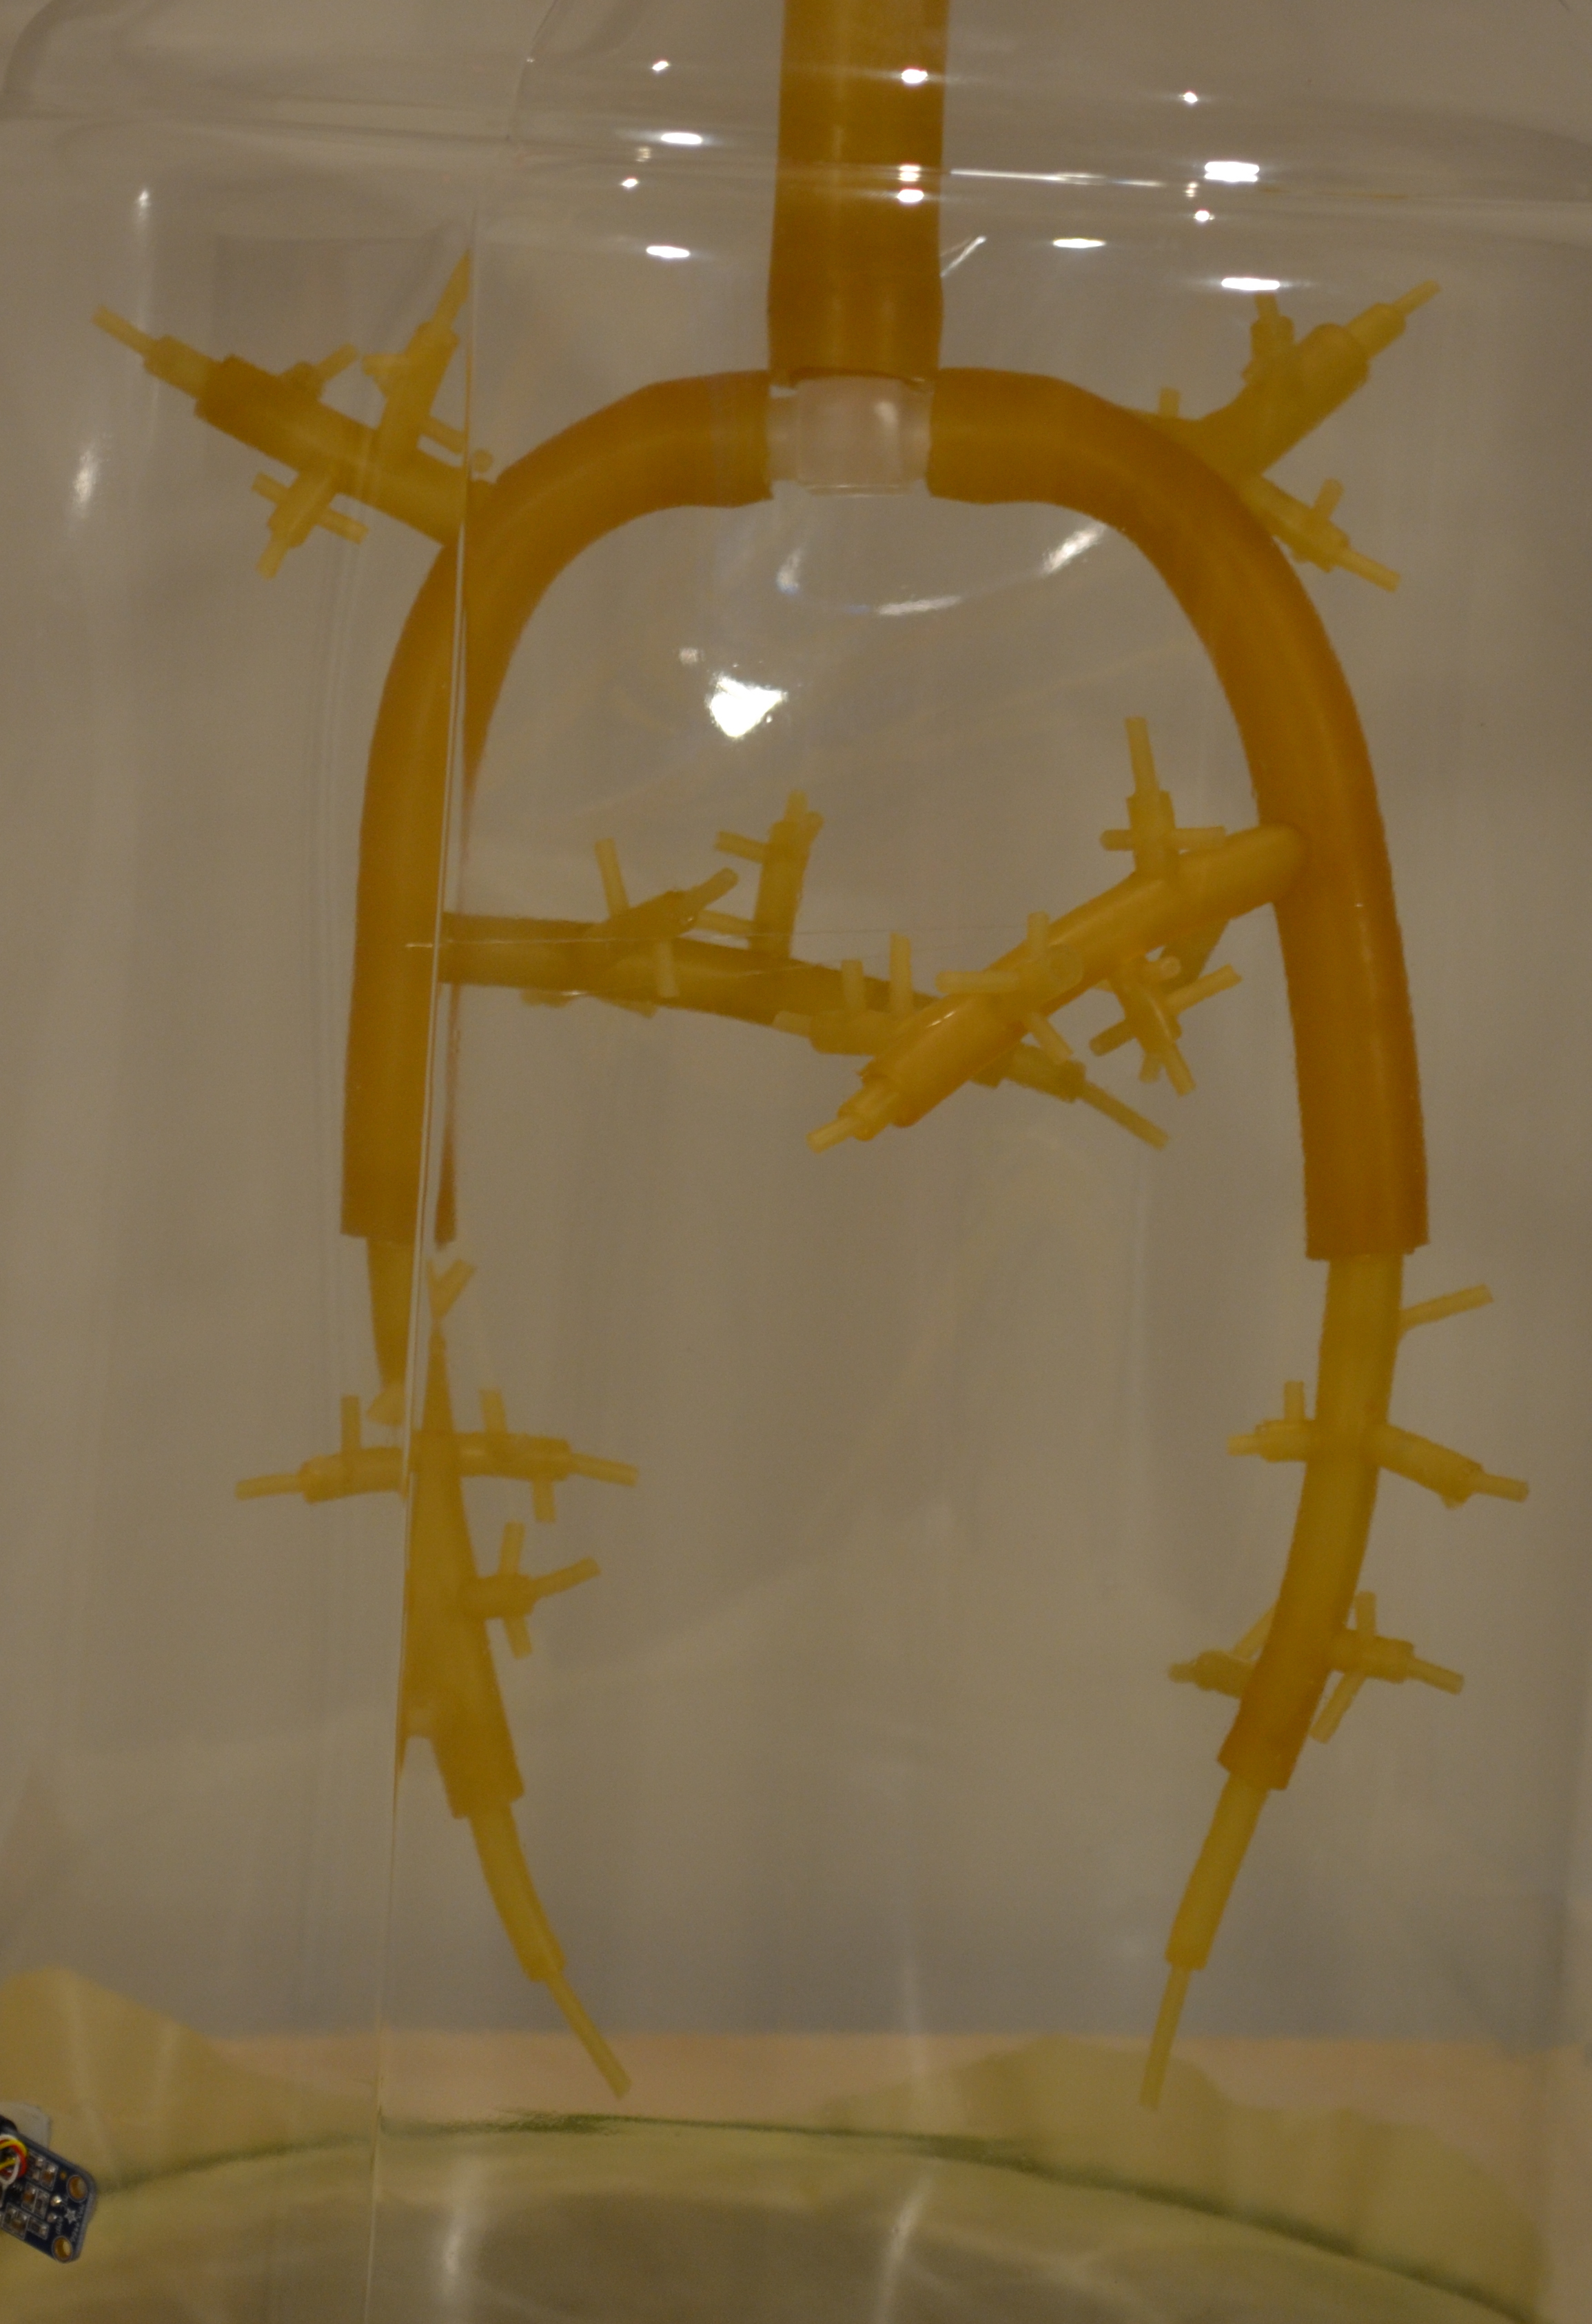
\includegraphics[width=0.5\textwidth]{images/closeupbronchialtree.JPG}
\caption{Bronchial tree.}
\end{figure}

% First, the interaction between the viewer and the breathing noises was much more intuitive. In prior user interviews we found that having the intensity of the breathing incerase in the presence of the viewer was more intuitive than the intensity of breath decreasing. This proved to be true as the change in intensity of breathing piqued viewers interest, causing them to approach the work. When they were vey close, the breathing reached its highest level of intensity and many viewers noted that they felt somewhat uncomfortable to be in such close proximity to the piece. In comparison, some users mentioned that at far away distances -- producing slow and relaxed breathing noises -- they found their own breath falling into a relaxing rythym and were enjoyed the meditative quatily produced. Overall, the auditory interaction consistently caused viewers to consider their own breath. 


\section{Discussion}

Initial research into the effects of disembodied breath revealed that the intensity and volume of the breathing noise has a large impact on the comfort level of the viewer. It was clear from the repetition of these trials in different settings that volume played major a role in the level of discomfort. Loud breathing noises inherently felt closer and more intimate than quieter noises. Cadence and pitch of breathing noises also appeared to have a lot of bearing on the emotion of the observer. A fast cadence of slightly higher pitch at higher volume was more noticeable and produced a higher degree of discomfort than a slower, softer breathing noise. 

In trials which involved playing noises of ``sick'' breathing noises, viewer response was much more intense. Results of these auditory trials were interesting because they illustrated just how sensitive the group had become to the noise of respiratory distress. While direct comparison is not possible, I wonder if these experiments would have had the same effect before the COVID-19 pandemic.  

These results were very helpful as I began to develop the digital breath generator. The ability to dynamically change the intensity and volume of breathing noises based on user proximity created a much more intuitive interaction between the viewer and the breathing noise. In prior user interviews I found that having the intensity of the breathing increase in the presence of the viewer was more natural than the intensity of breath decreasing. This proved to be true as the change in intensity of breathing piqued viewers interest, causing them to approach the work. When they were very close, the breathing reached its highest level of intensity and many viewers noted that they felt somewhat uncomfortable to be in such close proximity to the piece. In comparison, some viewers mentioned that at far away distances -- producing slow and relaxed breathing noises -- they found their own breath falling into a relaxing rhythm and were enjoyed the meditative quality produced. Overall, the auditory interaction consistently caused viewers to consider their own breath. 

While the variation in breath noises that could be produced using the initial trachea and diaphragm mechanism was very satisfactory, the look and feel of the mechanism had little relationship to the human body. Viewers noted that it was hard to relate the noised produced to the object itself. By making the movement of the diaphragm visible and creating an internal structure reminiscent of the bronchial tree I was able to draw viewers attention to the intended functionality of the work without the additional context of movement or sound. Upon seeing the bronchial structure many viewers immediately concluded that the work had to do with the lungs. This static visual cue really helped to enforce the intent of the interaction.

During user testing when the lever mechanism was activated viewers were extremely curious about the movement of the diaphragm. This simple motion was the most intuitive and seemed to produce the most natural reference to breath. Based on the sound emanating from the bronchial tree and trachea it was very clear that the motion of diaphragm was causing air to be forced out of the vessel. The look of the movement of the lever head through the latex diaphragm seemed both to attract and repel viewers. This slightly morbid curiosity was extremely effective at holding viewer's attention on the work.  

%The bronchial tree added an immediate visual indicator of the work's functionality while the addition of the clear chamber allowed the viewer to guess at the diaphragm's functionality.
\section{Further Work}

% emotion of breath
% mechanical complexity
% context


While the combination of mechanical breath and user interaction are core components of this exploration, they are not strictly necessary to continue exploring the emotion which can be conveyed through breath. The auditory trials in this investigation only scratched the surface of the nuanced emotion that breath can signify. I am curious to use this work as a platform to explore the narrative qualities of breath through viewer interaction. What kind of dialog can the work spark between itself and the viewer or between multiple viewers? What types of stories can the viewer intuit between themself and the work? These questions ultimately ask what range of emotion can be conveyed through the act of breathing.

Expanding on the mechanical techniques developed here, I hope to create a fully automated, mechanical version of this work. Combining the interactive qualities of the digital breath generator with the visual qualities of the mechanical trials will ultimately tie the core interaction and the kinetic intent of this work together. This investigation intended to pinpoint the relationship between what is natural and what is alive through the medium of movement. User testing revealed that the kinetic potential of this work was the most exciting part. However, this work is not yet living since it does not initiate the visible act of breathing.

By replacing the lever mechanism with a crank shaft -- a technique for translating circular motion into linear motion -- I hope to have fine grained control over the movement of the diaphragm and thereby the actuation of air through the work. This will then allow for further development and testing of the mechanical trachea. The modulation of breath does not end with the trachea however, and I hope to continue exploring the ways in which this sound can be manipulated. Perhaps the development of a mechanical pharynx, or larynx would follow. 

Finally, I am curious to investigate how the context of this work can be expanded beyond a traditional gallery space. One of the original questions this work intended to address, albeit obliquely, was how breath can be extended as a metaphor for humanity's relationship with the natural world. I believe it will be difficult to answer this question more specifically within the constraints of a gallery. Putting this piece in direct conversation with the natural world would expand the relationship of its breath beyond the viewer to the environment it inhabits. 


\section{Conclusion}


The primary objective of this work was to create a kinetic sculpture which appeared to be alive and breathing, thereby asking what it means for an non-living, artifical construct to breathe in a natural, life-like way. This objective was approached trough a combination of auditory and mechanical explorations. These investigations revealed that breath is a sensitive topic and can be interpreted as an indicator of many things. In addition to my intent of using breath as an indicator of life, I found that it is also a subtle and powerful indicator of emotion and health. The ongoing COVID-19 pandemic has certainly made us more attuned to the subtle changes in breath that signal respiratory distress.

The sound of breath can be used to great effect, however, these investigations revealed that the movement of breath is a much more intuitive signifier of life. The mechanical goal of this work was to isolate the components of the respiratory system which form the noise created by breathing and highlight their movement. The intensity of viewer's reactions to the mechanical system developed confirmed that the movement is just as powerful as sound in indicating life. 


Each human breath on this planet has moved us one step further into the Anthropocene and closer, some would argue to the end of nature. To conceptualize the impact of human activity on this planet is practically impossible, yet we find ourselves at a juncture where this definition is at the heart of nearly every social and political issue. Like James Prosek, we must all be wondering ``what can art provide in this time when our earth is indeed looking vulnerable to rapid and regrettable change induced by human influence?''\cite{prosek} If Art is a transcendent mechanism for collapsing the scales of Time and space we need it now more than ever to make sense of this recursively enormous question.


% Humans have created many mechanisms to mimic various aspects of the respiratory system for purposes ranging from medical devices, underwater exploration, to speech synthesis and more. Most of these devices are highly specialized and seek to mimic particular aspects of respiration such as oxygen delivery, or vocal modulation. These works rarely mimic the actual mechanics of the components of the human body responsible for respiration favoring more abstracted and efficient mechanical systems to achieve their goal. Using the freedom afforded by kinetic sculpture, this work attempts to blend a human-biomimetic approach -- highlighting the mechanical simplicity of the human body -- with a highly technical approach which allows for precise and complex control over the resulting breath. 
% clearly breath is a sensitive topic and can convey many things among them emotion, health etc
% this work confirmed that the movement of breath is a visual indicator of what it means to be alive
% as carl zimmer notes however, life cannot be categorized by one property, it perpetually depends on ...a system
% Using the human act of breathing as a lens, this work attempts to lay a foundation for inquiry into the relationship between what is considered to be natural and what is or has been alive. While the focus of this work is on a specifically human form of breath, respiration in broader context is omnipresent in living organisms and is therefore an apt biological process with which to address this question. This machine may breath in a natural way, but its appearance clearly identifies it as something which is purely artificial.


 
% Mark Dion
% Your question answers itself - the job of the artist-naturalist is precisely to interrogate the question of nature when it is subject to rapid change and its very definition is evolving in unprecedented ways.


% bring this back to the question of the relationship between what is natural and what is alive
% here is where I can cite some of the exciting reading I've done and talk about the big distinction of artificial and natural







% CONCLUSION:
% With each human breath on this planet we move deeper into the anthropocene.
% Respiration in breathing organisms is a visibly mechanical process. 
% 


% The root of my curiosity in addressing the boundary between what is natural and artificial is a desire to understand how creative practitioners can use the uncertainty surrouding thie distinction to generate reflection and consideration of humanity's place in the natural world. 


\cite{zimmer}




% why it's important to think about this in the context of humanity's relationship with the natural world


%\begin{figure}[h]
%
\includegraphics[width=3.31in]{figure.png}
%\caption{This is an example of figure caption. Note that all figures, and tables are to be referenced in the text. \copyright Respect Copyright.}
%\end{figure}
%
%\begin{figure*}
%
\includegraphics[width=\textwidth]{two-column-figure.png}
%\caption{Example of a double-column figure with caption. \copyright Respect Copyright.}
%\end{figure*}

\bibliographystyle{unsrt}
\bibliography{ms1report}

\section{Author Biography}
Lauria Clarke is an engineer and artist living in New York. She specializes in digital hardware design and kinetic sculpture and is always curious to learn more about humanity's relationship with the natural world.

% She completed a MS in Computer Engineering at Northeastern University in 2017 and is currently pursuing an MFA in Design and Technology at The Parsons School of Design. 

% aspires to be a chocolate fish fisherman for Ben and Jerry's.


\end{document}


% Masahiro Mori's 1970 essay prvided the framework for describing the confusing relationship between artifically created human-like robots and, as Mori calls us, real human beings. \cite{mori} This framework of thought has gained significant traction over the last 50 plus years as developments in technology have made it possiblt to mimic the human body with increasing accuracy. This definition has also been critical in the field of computer science as we consinute ot refine mahcine learning techniques which steadily approach the capacities of the uhman brain. This framework describes the point at which an artificial automaton approaches a point of being eeriely similar to a human being, creating a feeling of discomfort via the uncertainty of whether it is "real".

% For the lats fifty years this framework fo thought has been critical in describing technology's relationship with humanity. 

% Over the last *** years however, the fields of biodesign and bioart have increasingly been asking similar questions not about tchnology and humanity, but technology and nature. In light of the increasing environmental pressures of human imposed climate change, these questions are becoming increasingly urgent. Technology is now being used t oreplicate and mimic natural systems. As Donna Haraway noted in her paper, we must thin kbeyond the human. \cite{haraway} The capacity of our technology has surpassed the instinctually introspective and can now mimic what is natural outside of ourselves. This is a critical development and harkens back to mode indigenous ways of thinking - moving and working with natural systems, rather than in opposition to. 

% If our relationship with technology is extending beyond the human so to must our language. Mori's framework is distinctly human centric. How then do we apply this thinking to non-human natural world? Is Mori's valley merely a snaller depression within a much broader valley encompassing the whole of the natural world? Do humans deserve a place in that broader cintext? To frame this question more broadly, how do we, as human beings, distinguish between what is natural and what is atrificial? How is this distinction shifting as our techological capacity for the artifical increases at great cost to the natural world. 

%While its focus is on a specifically human foram of respiration, respiration in broader context is omnipresent in living organisms, thus providing a jumping off point for larger scope of inquiry into the relationship between what it means to be alive and what it means to be natural. Something about being alive. \cite{zimmer}
